                        %%%%%   PREAMBLE  %%%%%

\documentclass[11pt,spanish,a4paper,twoside]{article}

\usepackage[spanish,activeacute,es-noindentfirst]{babel}   % es-noindentfirst: no activa la sangr�a del primer p�rrafo tras un t�tulo
\usepackage{amssymb,amsfonts}
\usepackage{amsmath}             %  Para las f�rmula matem�ticas
\usepackage[latin1]{inputenc}    %  Permite escribir los acentos

\usepackage{fancyhdr}
\renewcommand{\headrulewidth}{0pt}  %  l�nea horiz. bajo el encabezado
\renewcommand{\footrulewidth}{0pt}  %  l�nea horiz. sobre el pie

\usepackage{makeidx}

% \usepackage{times}
% \usepackage[OT1,T1]{fontenc}

\usepackage{palatino}
% palatino: una fuente excelente, pero si sale
% mal en el .pdf descomentar las dos l�neas anterires
% y comentar �sta.

% \usepackage{charter}

\usepackage{vmargin}
\setpapersize{A4}
\setmarginsrb{2.5cm}{2cm}{2.5cm}{2cm}%
{1cm}{1cm}%
{1cm}{1cm}


\usepackage{graphicx}
\usepackage{color}       % Para el color de las fuentes
% \usepackage{lettrine}    % Letra capital
\usepackage{enumerate}   % Entorno enumerate mejorado
\usepackage{mdwlist}     % Entorno descripcion mejorado
\usepackage[amsthm,hyperref,thref]{ntheorem}
%\usepackage{paralist}


\parskip 0.15cm          % Queda mejor pero mas paginas

                        %%%%%   HYPERREF  %%%%%

\usepackage{hyperref}        %  Hiperv�nculos
\hypersetup{                 %  Hiperv�nculos setup
    bookmarksopen=false,
    bookmarksnumbered=true,
    pdfpagemode=UseOutlines,  % None, UseThumbs, UseOutlines (show bookmarks), FullScreen
    colorlinks=true,     % color link text, not a box around them.
    linkcolor=black,      % color for normal internal links.
    anchorcolor=black,   % color for anchor text.
    citecolor=blue,      % color for bibligraphical citations in text.
    filecolor=black,     % color for URLs which open local files.
    menucolor=black,     % color for Acrobat menu items.
%     pagecolor=black,     % color for links to other pages.
    urlcolor=blue,      % color for linked URLs.
    breaklinks=false,    % Allows link text to break across.
    pdfstartview={FitBH},
    pdfview={FitBH},
    %hyperindex=true,
    pageanchor=false
}

% Para el �ltimo
% En realidad, no pasa eso, pero si no pongo "false" tira errores.
%    Determines whether every page is given an implicit
%    anchor at the top left corner. If this is turned off,
%    \tableofcontents will not contain hyperlinks.

% El pen�ltimo me tira un warning pero dejarlo sin comentar     % Hiperreferencias

\usepackage{url}

% \usepackage{longtable}
% \usepackage{supertabular}


% \usepackage{tikz}
% \usepackage{pgf}
% \usepackage{wrapfig}

% \usepackage{placeins}   % Placeins.sty keeps floats "in their place", preventing them from floating past
                        % a "\FloatBarrier" command into another section. To use it, declare
                        % "\usepackage{placeins}" and insert "\FloatBarrier" at places that floats
                        % should not move past, perhaps at every "\section" (en "command.tex")

%% Entorno Descripci�n. En tres sabores:
    %% 1. El m�s general
    \newenvironment{descripcion}[2]%
    {\begin{basedescript}{\desclabelwidth{#2}}%
    \item[#1]}%
    {\end{basedescript}}%

    %% 2. Como poner en negrita (tambi�n parecido a section* pero puedo seguir en la misma l�nea)
    \newenvironment{descripcion0}[1]%
    {\begin{basedescript}{\desclabelwidth{-1ex}}%
    \item[#1]}%
    {\end{basedescript}}%

    %% 3. Con 1.25cm de tama�o
    \newenvironment{descripcion1}[1]%
    {\begin{basedescript}{\desclabelwidth{1.25cm}}%
    \item[#1]}%
    {\end{basedescript}}%

    %% Entorno para citar texto, 80% del tama�o (10% de cada lado)
      \newenvironment{citetext}{%
      \def\leftmargini{0.1\textwidth}%
      \def\rightmargini{0.1\textwidth}%
      \vspace*{-0.35cm}%
      \begin{quotation}\parskip 0.15cm\guillemotleft}%
      {\guillemotright\end{quotation}\vspace*{0.1cm}}


      %% Sin � (caso especial de citetext)
      \newenvironment{citetext_sin_right}{%
      \def\leftmargini{0.1\textwidth}%
      \def\rightmargini{0.1\textwidth}%
      \vspace*{-0.35cm}%
      \begin{quotation}\parskip 0.15cm\guillemotleft}%
      { \end{quotation}\vspace*{0.1cm}}



\newcommand{\subsubseccion}[1]{\subsubsection*{#1}\addcontentsline{toc}{subsubsection}{#1}}




\newcommand{\cleartoevenpage}{%   Similar a \cleardoublepage
    \clearpage
    \ifodd\thepage
        \newpage
    \else
        \newpage
        ~ \\
        \newpage
    \fi
}




\newcommand{\refEQ}[1]{{\color{red} (\ref{#1})}}


\makeindex

\begin{document}
    \pagestyle{headings}
                                           %%% TITULO %%%

\pagestyle{empty}   % para que no tenga n�mero
                    % (�ste es el motivo por el
                    %  cu�l no uso "\maketitle")

% \vspace*{-1.65 cm}
 \begin{center}
   \begin{Large}
%          Online Mathematical Handwriting Recognition
         \textbf{Online Handwriting Recognition}
   \end{Large}
 \end{center}


\vspace*{1.65 cm}
\begin{center}
  \begin{Large}
    \textit{Tesina de Grado
    \vspace*{0.1 cm} \\
    \begin{footnotesize}Agosto 2011    \end{footnotesize}
    }
  \end{Large}
\end{center}


\vspace*{1.65 cm}
\begin{center}
  \begin{Large}
   \textsc{Pablo Speciale}
  \end{Large}
\end{center}


\vspace*{1.65 cm}
\begin{center}
    
\includegraphics[scale=0.04]{imagen/logo_fceia.pdf}
    \hspace*{5cm}
    
\includegraphics[scale=0.25]{imagen/logo_unr.pdf}
\end{center}


\vspace*{0.65 cm}
\begin{center}
\textit{
Lic. en Cs. de la Computaci�n \\
Facultad de Ciencias Exactas, Ingenier�a y Agrimensura \\
Universidad Nacional de Rosario}
\end{center}


\vspace*{3.5cm}
\textbf{Director}: Dr. Juan Carlos Gomez\footnote{Director del grupo \textit{Procesamiento de Se�ales Multimedia} del CIFASIS}

% \vspace{0.5cm}
\textbf{Co-director}:  Dr. Pablo Granitto\footnote{Director del grupo \textit{Aprendizaje Automatizado y Aplicaciones} del CIFASIS}


\newpage




% 
% 
% \topmargin 0 truecm
% 
% \pagestyle{empty}
% 
% \begin{center}
% 
% \vskip -3.0cm
% {\LARGE \sf {\huge mcBrief}: un descriptor local de features \\ para im�genes color} \\
% 
% \vspace{4.0cm}
% {\Large \sf Tesina de grado}
% 
% \vspace{1.5cm}
% {\Large Autor: Daniel Moreno}
% 
% \vspace{0.5cm}
% {\Large Director: Mario E. Munich}
% 
% \vspace{2.4cm}
% {\large \sf Julio 2011}
% 
% \vspace{2.5cm}
% 
% \begin{figure}[h]
% \begin{center}
% \includegraphics[height=1.6cm]{logo_lcc.png}
% \end{center}
% \end{figure}
% 
% \begin{figure}[h]
% \begin{center}
% \includegraphics[height=1.6cm,width=1.6cm]{LogoUNR.png}
% \end{center}
% \end{figure}
% 
% 
% {\it Lic. en Cs. de la Computaci�n \\
% Facultad de Ciencias Exactas, Ingenier�a y Agrimensura \\
% Universidad Nacional de Rosario }
% 
% 
% \end{center}
%     \section*{Prefacio}

\subsection*{Grupo de Trabajo}
\noindent
El siguiente proyecto involucra t�picos del �rea del conocimiento de Aprendizaje Automatizado (Machine Learning) y de Procesamiento de Se�ales. Se trabajar� con Dr. Pablo Granitto, director del grupo \textit{Aprendizaje Automatizado y Aplicaciones} del CIFASIS, y con Dr. Juan Carlos G�mez, director del grupo \textit{Procesamiento de Se�ales Multimedia} del CIFASIS.

                            %%%%%   INDICE  %%%%%

\setcounter{page}{1}
\thispagestyle{empty}
\pagenumbering{roman}        % N�meros de p�ginas en Romano

\pagestyle{fancy}
\fancyhf{}                   % Borrar todos los ajustes
\fancyhead[RO,RE]{\scshape{\thepage}}
\fancyhead[LO]{\scshape{�ndice General}}
\fancyhead[LE]{\scshape{�ndice General}}

\pdfbookmark[0]{�ndice General}{tit}       %Agrega "�ndice General"' al bookmark.

\tableofcontents
\clearpage

                            %%%%%   ESTILO  %%%%%

\renewcommand{\headrulewidth}{0pt}  %  l�nea horiz. bajo el encabezado
\renewcommand{\footrulewidth}{0pt}  %  l�nea horiz. sobre el pie

\pagenumbering{arabic}

%
%  Simple faz
%
\pagestyle{fancy}
\fancyhf{}                   % Borrar todos los ajustes
\fancyfoot[C]{\thepage}
% \fancyhead[RO,RE]{\scshape{\thepage}}  % N�meros de p�gina en las esquinas de los encabezados
\renewcommand{\sectionmark}[1]{
    \fancyhead[RO]{\begin{footnotesize}\thesection.\ \scshape{#1}\end{footnotesize}}
    \fancyhead[RE]{\begin{footnotesize}\thesection.\ \scshape{#1}\end{footnotesize}}
    \renewcommand{\headrulewidth}{0.1pt}
}
\renewcommand{\subsectionmark}[1]{
    \fancyhead[RE]{\begin{footnotesize}\thesubsection.\ \scshape{#1}\end{footnotesize}}
}


%
%  Doble faz
%
% \pagestyle{fancy}
% \fancyhf{}                   % Borrar todos los ajustes
% \fancyfoot[C]{\thepage}
% % \fancyhead[RO,LE]{\begin{small}\thepage\end{small}}  % N�meros de p�gina en las esquinas de los encabezados
% \renewcommand{\sectionmark}[1]{
%     \fancyhead[RO]{\begin{footnotesize}\thesection.\ \scshape{#1}\end{footnotesize}}
%     \fancyhead[LE]{\begin{footnotesize}\thesection.\ \scshape{#1}\end{footnotesize}}
%     \renewcommand{\headrulewidth}{0.1pt}
% }
% \renewcommand{\subsectionmark}[1]{
%     \fancyhead[RE]{\begin{footnotesize}\thesubsection.\ \scshape{#1}                   \end{footnotesize}}
% }


%% Para los perzonalizar itemize
\renewcommand{\labelitemi}{$\bullet$}
\renewcommand{\labelitemii}{$\ast$}


% % A more convenient way to stop floats at section boundaries is to change
% % the definition of "\section" to include "\FloatBarrier", at the beginning
% \let\oldsection\section
% \renewcommand{\section}{\FloatBarrier\oldsection}


% % Util para ser impreso. Hace que las secciones comiencen desde una p�gina impar
% % similar a \cleardoublepage
% \let\oldsection\section
% \renewcommand{\section}{\cleartoevenpage\oldsection}


\let\oldsection\section
\renewcommand{\section}{\clearpage\oldsection}


\def\tablename{Tabla} % Cambia "Cuadro" por "Tabla"


% Links internos en rojo
\hypersetup{
    linkcolor=red,
}

    \pagestyle{fancy}
    
    \section{Introducci�n}

\subsection*{Motivaci�n}
\noindent
Poder escribir en dispositivos electr�nicos es factible actualmente, sobre todo con la llegada de las Tablet PC, pizarras el�ctricas, celulares touch-screen y las pantallas t�ctiles. Tambi�n cabe destacar algunos e-Readers que permiten la escritura, convirti�ndose en \textit{papel electr�nico}. La escritura se realiza generalmente con un \textit{stylus} (l�piz), abriendo la puerta a nuevas interacciones m�s all� del teclado y mouse. En la figura \ref{tabletas}, puede apreciarse una variedad de dispositivos que permiten la escritura con l�piz.
\begin{figure}[!htbp]
 \centering
 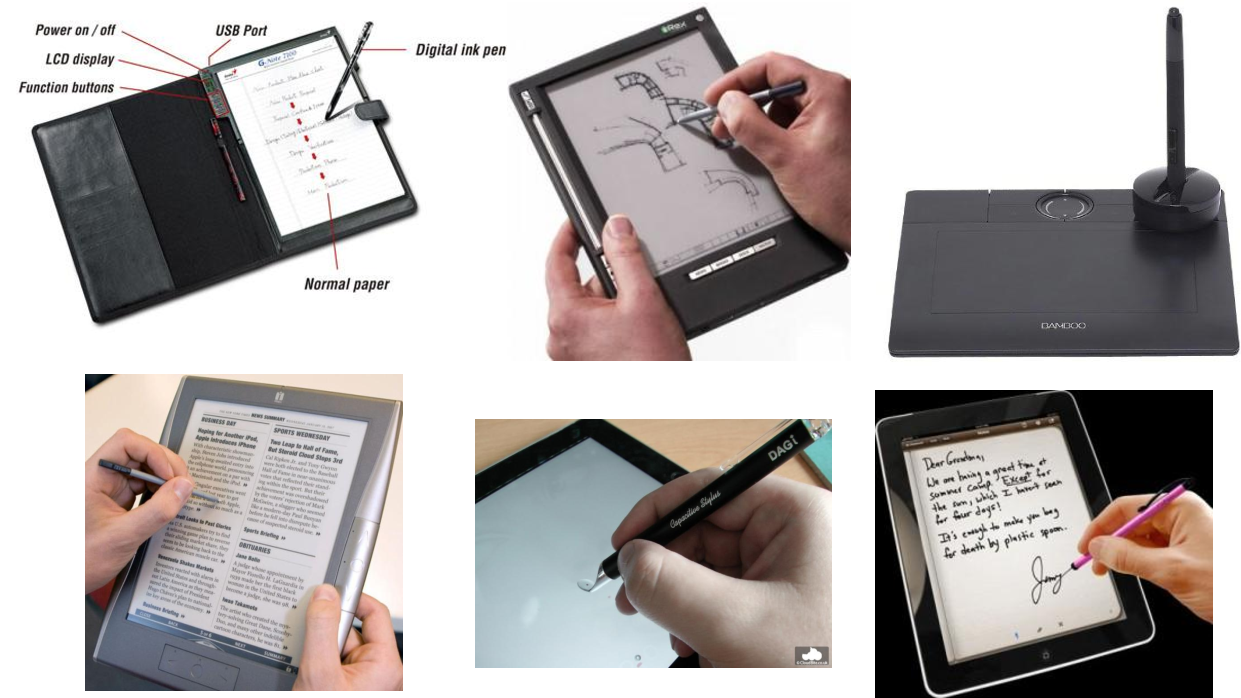
\includegraphics[scale=0.70]{imagen/tabletas.pdf}
 \caption{Tabletas}
 \label{tabletas}
\end{figure}


\vspace*{-1ex}
\subsection*{Online vs Offline Recognition}
\label{Fundamentos}

% \subsubsection*{On-line vs Off-line}
\noindent
A diferencia del enfoque \textit{Offline} de handwriting recognition, el cual pretende reconocer caracteres a partir de una imagen, el enfoque \textit{Online} intenta el reconocimiento a partir de trazos. Ambos enfoques est�n esquem�ticamente representados en la figura \ref{fig:off|on-line}.
\begin{figure}[!htbp]
 \centering
 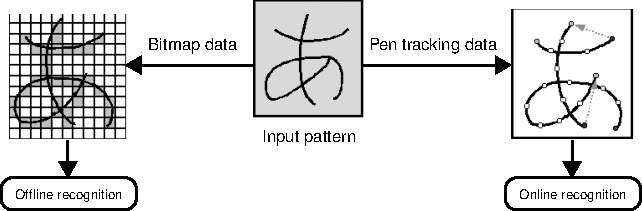
\includegraphics[scale=0.85]{imagen/off|on-line.pdf}
 \caption{Offline vs Online.}
 \label{fig:off|on-line}
\end{figure}

Como puede verse, se posee el orden en que cada uno de los puntos fue escrito. As�, es posible diferenciar distintos estilos de escrituras, a pesar de que el resultado final puede que sea el mismo. . La utilizaci�n de un stylus en un dispositivo electr�nico permite usar el enfoque online.



\subsubsection*{Handwriting recognition}
\noindent
En el an�lisis de Handwriting para contenido matem�tico se reconocen 4 etapas, como se destaca en \cite{CommunicatingMathematics}:
% colecci�n de trazos (digital ink), reconocimiento de caracteres, an�lisis estructural y determinaci�n de sem�ntica.

\begin{enumerate}[A.]

 \item \textbf{Colecci�n de trazos}

Un caracter puede ser escrito con un s�lo trazo (\textit{Single-Stroke}) o con muchos (\textit{Multi-Stroke}), ver figura \ref{fig:single|multi-stroke}. El problema de determinar qu� trazos pertenecen a qu� caracteres es llamado \textit{Stroke grouping}.
\begin{figure}[!htbp]
 \centering
 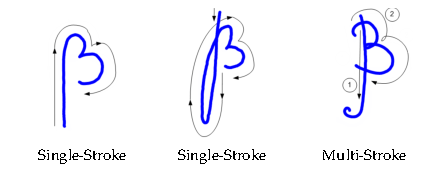
\includegraphics{imagen/single|multi-stroke.pdf}
 \caption{Izquierda y centro caracter Single-Stroke. Derecha Multi-Stroke.}
 \label{fig:single|multi-stroke}
\end{figure}


 \item \textbf{Reconocimiento de caracteres}

El reconocimiento tiene 3 etapas:
    \begin{enumerate}[1.]
    \item \textit{Preproceso}

    El preprocesado primero elimina el ruido frecuentemente presente al principio y final de cada trazo. Luego, se normaliza por \textit{resampling} y \textit{resizing}. Resampling ayuda a unificar distancias entre los puntos, y resizing asegura que el tama�o del caracter escrito no afecte al resultado del reconocimiento.

    \begin{figure}[!htbp]
    \centering
    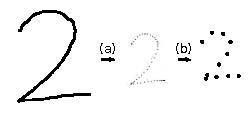
\includegraphics{imagen/preprocesing.pdf}
    \label{fig:preprocesing}
    \caption{(a) Suavizado y resizing, (b) luego resampling }
    \end{figure}


    \item \textit{Extracci�n de caracter�sticas (Feature extraction)}

    En este paso se extraen caracter�sticas (feature) de los trazos. Hay varios tipos de features: los relativos a apariencia que incluye, por ejemplo, proporci�n entre la altura y ancho; los relativos a propiedades geom�tricas, como ser la cantidad de loops e intersecciones; los relativos al estilo de escritura, como la direcci�n y cantidad de strokes.

    Estos features son usados como criterio para podar el �rbol de modelos, dejando una cantidad peque�a de clases a examinar, incrementando la performance del reconocimiento. Por ejemplo, en el caso de escribir ``$\ell$'' o ``$\alpha$'', solo se considerar�n los modelos que contienen un �nico loop.


    \item \textit{Matching}

    La etapa final del reconocimiento es el matching de la entrada con los modelos en una base de datos. Despu�s de que los features podaron el �rbol de modelos, es necesario lidiar con solo una fracci�n de la colecci�n. Se pueden citar algoritmos como \textit{Elastic Matching} \cite{ElasticMatching} o \textit{Legendre-Sobolev} \cite{LegendreSobolevComp, OnlineStrokeModeling}.

    \end{enumerate}


% \newpage
    \item \textbf{An�lisis estructural}

Como la entrada se espera que sea matem�tica, adem�s de reconocer cada caracter individual, tambi�n se tienen que interpretar su posici�n y rol en la expresi�n. Primero, se considera solo la posici�n relativa de los caracteres, sin determinar su sem�ntica, como se ve en el ejemplo representado en la figura \ref{fig:layout_trees}.
\begin{figure}[!htbp]
 \centering
 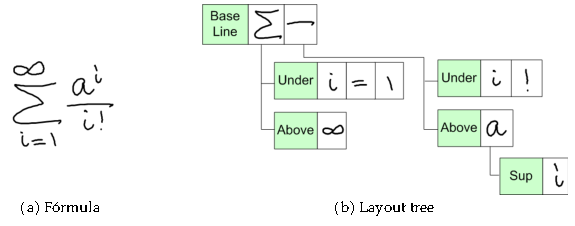
\includegraphics{imagen/layout_trees.pdf}
 \caption{Representaci�n de la f�rmula manuscrita y su correspondiente Layout.}
 \label{fig:layout_trees}
\end{figure}

Luego, se marcan expl�citamente decimales, operadores, fracciones, etc. Cada nodo en el �rbol es asignado a un rol en la expresi�n. Se intenta distinguir entre nombres de funciones y de variables, entre multiplicaciones impl�citas de aplicaci�n de funciones, etc. %Esta etapa es dif�cil y requiere sem�ntica profunda.



\item \textbf{Extracci�n de contenido matem�tico}

El �rbol construido despu�s del an�lisis estructural ya posee sem�ntica y puede ser transformado directamente a \LaTeX~ o MathML \cite{MathML}.


\end{enumerate}


%     \section{Posibles Aplicaciones}

\subsection{Reconocimiento de f�rmulas matem�ticas}

Como hemos indicado anteriormente, existe una variedad importante de dispositivos electr�nicos en los que se puede usar un l�piz. Sin embargo, todav�a no hay una aplicaci�n sobresaliente para tales dispositivos. El usuario ve al stylus como un mouse sofisticado. Vemos en la matem�tica una aplicaci�n que puede cambiar el estado actual. No s�lo escribir en matem�tica sino tambi�n trabajar con expresiones, ya que actualmente existen poderosos sistemas de c�lculo simb�lico, como Maple \cite{Maple}.

Una obvia motivaci�n es el hecho de que escribir matem�tica en una computadora es problem�tico. Por ejemplo, la expresi�n:
\begin{figure}[!htbp]
    \centering
    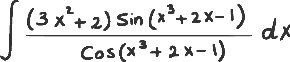
\includegraphics{imagen/formula.pdf}
\end{figure}

\noindent
es m�s natural que escribir en \LaTeX:
\vspace*{-1ex}
\begin{footnotesize}\begin{verbatim}
                    \int {\frac { \left( 3\,{x}^{2}+2 \right)
                                  \sin \left( {x}^{3}+2\,x-1 \right) }
                                { \cos \left( {x}^{3}+2\,x-1 \right) }
                         } ~ dx
\end{verbatim}\end{footnotesize}


En el campo de reconocimiento de escritura matem�tica hay un n�mero de desaf�os a sortear. A nivel de \textbf{s�mbolos}, existen muchos que son similares y no existe un alfabeto peque�o como lo tiene un lenguaje natural. A nivel de \textbf{entrada}, la segmentaci�n de s�mbolos matem�ticos es considerablemente m�s complicada. A nivel de construcci�n de \textbf{f�rmulas v�lidas}, el texto por naturaleza es unidimensional pero expresiones matem�ticas son bidimensionales, haciendo dif�cil determinar una l�nea de referencia (\textit{baseline}) apropiada. A nivel del \textbf{renderizado}, el dibujado de s�mbolos matem�ticos no es trivial. A nivel de \textbf{interacci�n}, el stylus es un dispositivo nuevo y la interacci�n hombre-computadora tiene que repensarse para que sea eficaz.


\subsubsection*{An�lisis estructural}

Como la entrada se espera que sea matem�tica, adem�s de reconocer cada caracter individualmente, tambi�n se tienen que interpretar su posici�n y rol en la expresi�n, ver figura \ref{fig:layout_trees}.
\begin{figure}[!htbp]
    \centering
%     \vspace*{-0.2cm}
    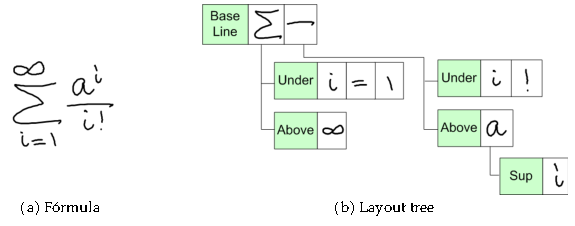
\includegraphics{imagen/layout_trees.pdf}
%     \vspace*{-0.3cm}
    \caption{Representaci�n de la f�rmula manuscrita y su correspondiente Layout.}
    \label{fig:layout_trees}
\end{figure}



\subsection{Reconocimiento de firmas}
Un campo muy interesante, donde se podr�a aplicar los m�todos mencionados en este trabajos, es el de verificaci�n de firma. Pueden verse ejemplos de firma en \ref{fig:firmas}. Se intentar� utilizar las representaciones por polinomios ortogonales descripta, para determinar si caracterizan lo suficientemente bien a las firmas como para ser usadas en este campo.
    \begin{figure}[!htbp]
    \centering
    
\includegraphics[scale=0.6]{imagen/firmas.pdf}
    \caption{Ejemplos de firmas}
    \label{fig:firmas}
    \end{figure}


\subsection{Reconocimiento de partituras musicales}
Otra aplicaci�n a considerar es el reconocimiento de notaci�n musical, como puede verse en la figura \ref{fig:partitura}. No se ha encontrado muchos sobre este tipo de reconocimiento usando el enfoque online.
    \begin{figure}[!htbp]
    \centering
    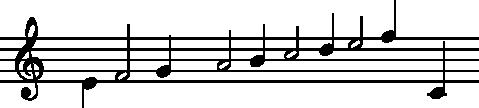
\includegraphics[scale=0.9]{imagen/Sheet_music.pdf}
    \caption{Partitura}
    \label{fig:partitura}
    \end{figure}



\bibliography{bibliografia} % indica el archivo de bibliograf�a
\bibliographystyle{pablo}   % indica el estilo de la bibliograf�a.
                            % Otros estilos (en orden de pref.): unsrt, alpha, plain, abbrv

\end{document}